\newpage
\section{Resoconto delle attività di verifica}
\subsection{Attività di analisi dei requisiti}

Dopo aver redatto tutti i documenti presenti nella Revisione dei Requisiti, il team ha svolto le attività di verifica su di essi e sui processi analizzati. I documenti sono stati sottoposti al processo di analisi statica definito nel documento \NdP{}.
Prima è stata utilizzata la tecnica del Walkthrough, segnalando gli errori incontrati tramite una lettura approfondita in un'apposita lista presa in carico dal \ver{} per attuare la correzione del documento. In seguito la stessa lista è stata utilizzata per la tecnica dell'Inspection, che è servita ad individuare la presenza di nuovi errori utilizzando il confronto della lista di quelli commessi in precedenza.
In seguito i documenti sono stati interamente verificati secondo le metriche descritte nell'Appendice~\nameref{AppB:metric} e sono stati riportati i risultati ottenuti.

\subsection{Attività di analisi dei requisiti in dettaglio}

In questo periodo di attività, il team si è impegnato a colmare le proprie lacune tecnologiche necessarie allo svolgimento del progetto. Parallelamente, si mira a consolidare ed ampliare i requisiti richiesti dal sistema e a migliorare il documento di AnalisiDeiRequisiti v1.0.0 attuando le correzioni in base all’esito della Revisione dei Requisiti; vengono inoltre corretti e verificati anche gli altri documenti, secondo le modalità descritte in precedenza. 


\subsection{Attività di prototipazione}
Questo periodo è caratterizzato dalla realizzazione di un prototipo utilizzando le tecnologie necessarie, con lo scopo di comprendere pienamente il dominio tecnologico del progetto attraverso la realizzazione dei casi d’uso essenziali e ritenuti
significativi per la buona riuscita del prodotto finale. Sono inoltre incrementati quasi tutti i documenti.


\subsection{Verifica dei processi}
\subsubsection{Schedule Variance}
Nel seguente grafico vengono riportati i valori ottenuti calcolando la Schedule Variance sui tempi di stesura di ogni documento rispetto ai tempi prefissati nel \PdP{}:

\begin{figure}[h!]
	\centering
	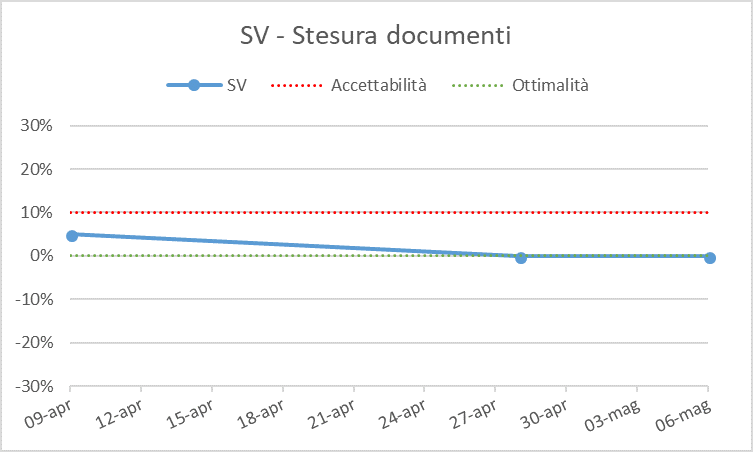
\includegraphics[scale=0.75]{img/Grafici/SV-Documenti.png}
		\caption{Schedule Variance sul processo di stesura dei documenti.}
	\label{fig:SV-Documenti}
\end{figure}
 
	Il grafico evidenzia come la schedule variance calcolata sul processo di documentazione, inizialmente solo entro il livello di accettabilità, si sia stabilizzata negli ultimi due periodi sul livello di ottimalità.

\subsubsection{Cost Variance}
Il calcolo della Cost Variance sul processo di documentazione ha portato il seguente risultato: 

\begin{figure}[h!]
	\centering
	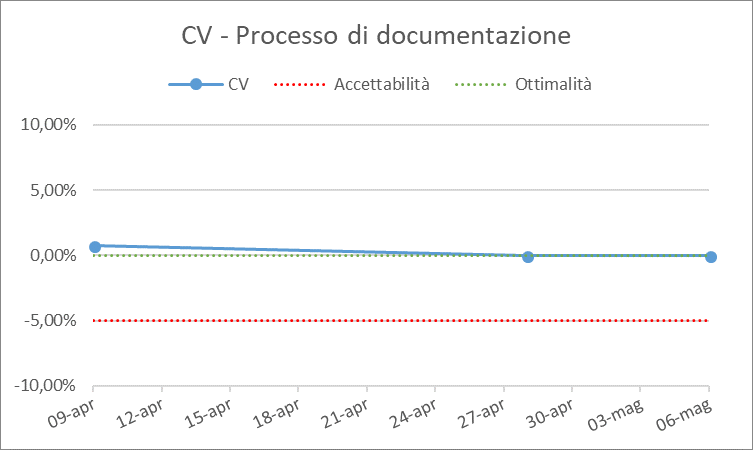
\includegraphics[scale=0.75]{img/Grafici/CV-S-Documenti.png}
	\caption{Cost Variance per il processo di documentazione.}
	\label{fig:CV-Documenti}
\end{figure}

	Il grafico evidenzia che la cost variance calcolata sul processo di documentazione è rimasta sempre entro i limiti di ottimalità.
	
\subsection{Verifica dei documenti}
\subsubsection{Schedule Variance}
Nel seguente grafico vengono riportati i valori ottenuti calcolando la Schedule Variance sui tempi di verifica di ogni documento rispetto ai tempi prefissati nel \PdP{}:

\begin{figure}[h!]
	\centering
	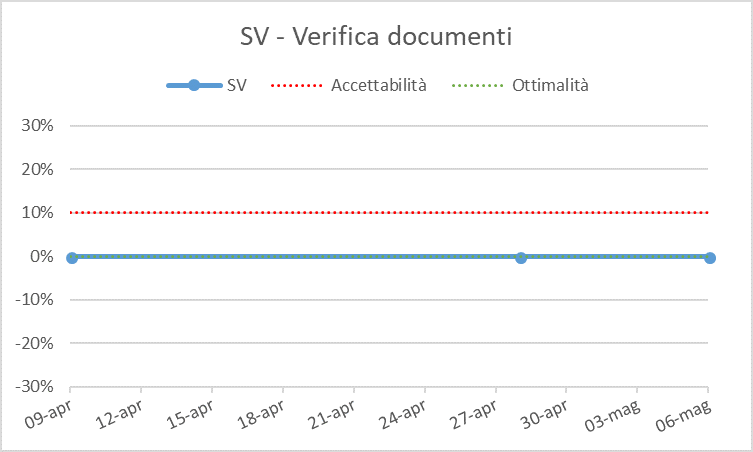
\includegraphics[scale=0.75]{img/Grafici/SV-VerDocumenti.png}
	\caption{Schedule Variance per la }
	\label{fig:SV-VerDocumenti}
\end{figure}

Il grafico evidenzia che la schedule variance calcolata sul processo di verifica della documentazione è rimasta sempre entro i limiti di ottimalità.


\subsubsection{Cost Variance}
Il calcolo della Cost Variance sul processo di verifica ha portato il seguente risultato: 

\begin{figure}[h!]
	\centering
	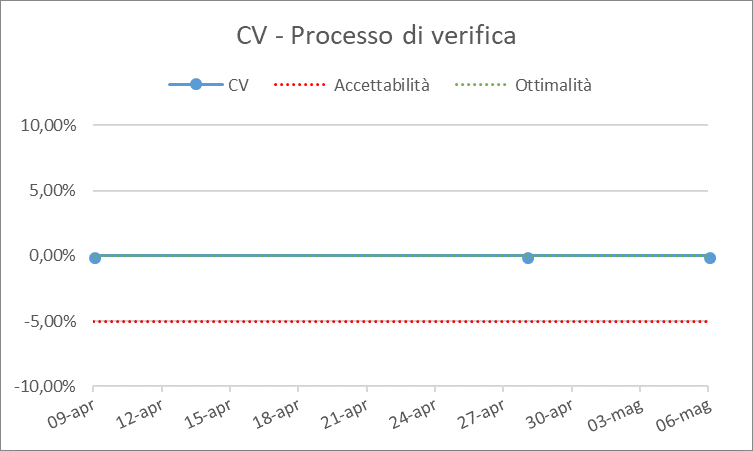
\includegraphics[scale=0.75]{img/Grafici/CV-V-Documenti.png}
	\caption{Cost Variance per il processo di verifica.}
	\label{fig:CV-VerDocumenti}
\end{figure}

Il grafico evidenzia che la cost variance calcolata sul processo di verifica, è rimasta sempre entro i limiti di ottimalità.


\subsubsection{Errori ortografici}
Durante l'ultima verifica, sono stati rilevati all'interno dei vari documenti alcuni errori ortografici, il cui numero è specificato nel seguente grafico:

\begin{figure}[h!]
	\centering
	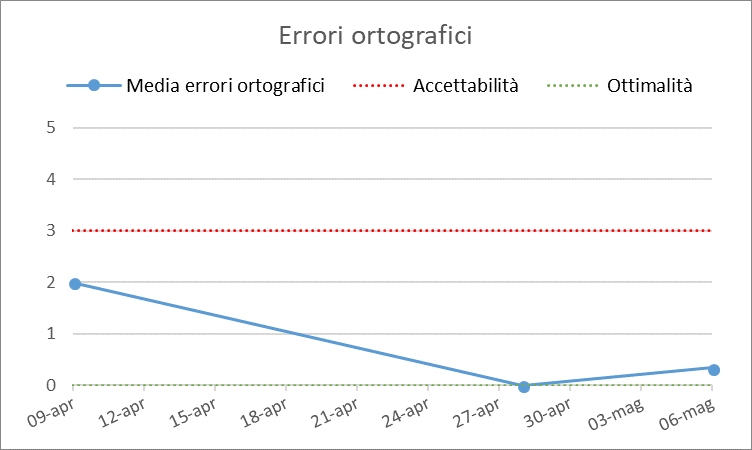
\includegraphics[scale=0.6]{img/Grafici/Errori_orto.png}
	\caption{Media degli errori ortografici.}
	\label{fig:Errori_orto}
\end{figure}

Il grafico evidenzia che la il numero medio di errori ortografici, è rimasto sempre entro i limiti di accettabilità.

\clearpage

\subsubsection{Errori concettuali}

Durante l'ultima verifica, sono stati rilevati all'interno dei vari documenti alcuni errori concettuali, il cui numero è specificato nel seguente grafico:

\begin{figure}[h!]
	\centering
	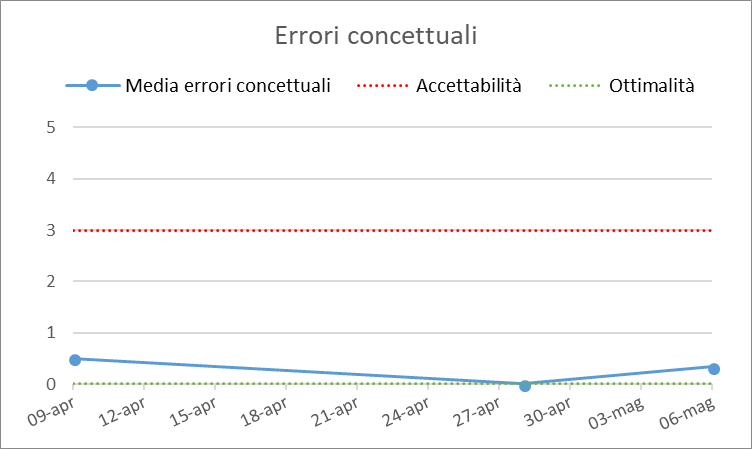
\includegraphics[scale=0.6]{img/Grafici/Errori_conce.png}
	\caption{Media degli errori concettuali}
	\label{fig:Errori_conce}
\end{figure}

Il grafico evidenzia che la il numero medio di errori concettuali è rimasto sempre entro i limiti di accettabilità.

\subsubsection{Errori di forma}

Durante l'ultima verifica, sono stati rilevati all'interno dei vari documenti alcuni errori forma, il cui numero è specificato nel seguente grafico:

\begin{figure}[h!]
	\centering
	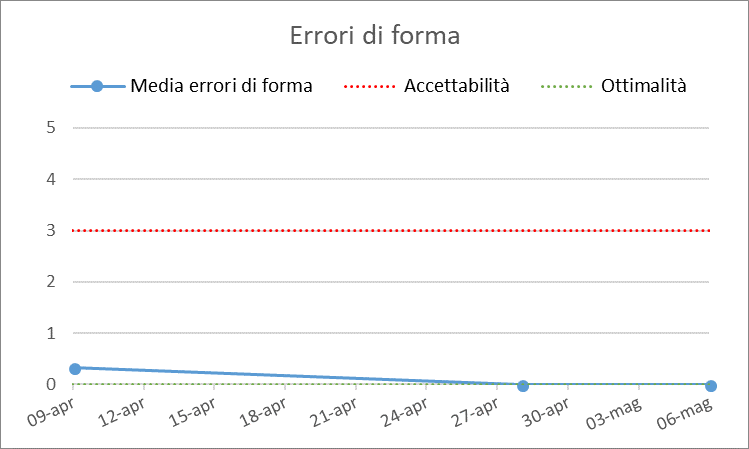
\includegraphics[scale=0.6]{img/Grafici/Errori_forma.png}
	\caption{Media degli errori di forma.}
	\label{fig:Errori_forma}
\end{figure}

Il grafico evidenzia che la il numero medio di errori di forma è rimasto sempre entro i limiti di accettabilità.
\newpage

\subsubsection{Indice Gulpease}

Tutti i documenti consegnati sono stati sottoposti al calcolo dell'Indice Gulpease per valutarne il grado di leggibilità, il quale è riportato nel seguente grafico:

\begin{figure}[h!]
	\centering
	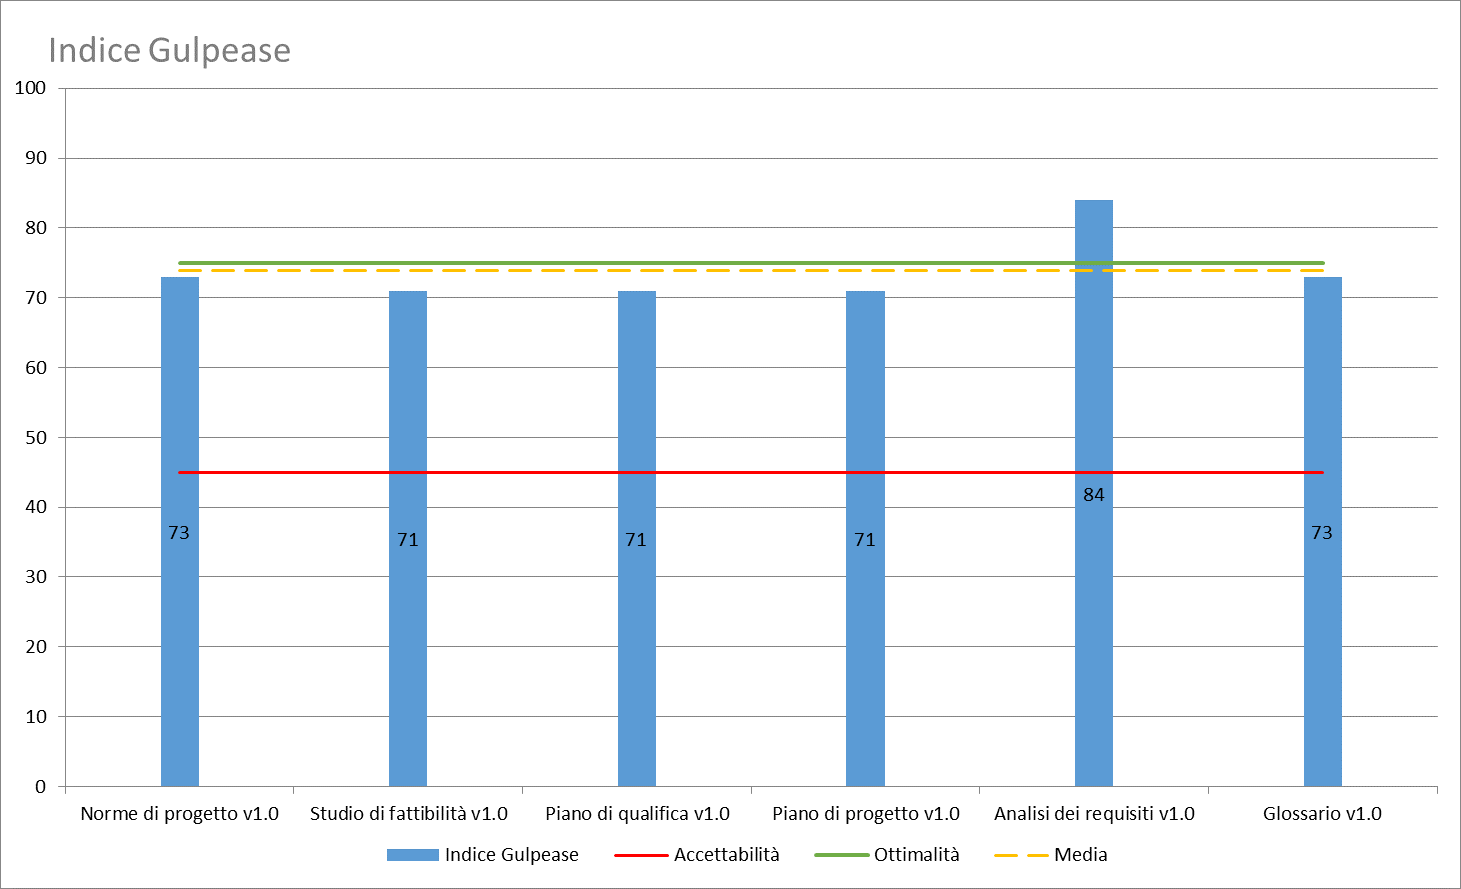
\includegraphics[scale=0.6]{img/Grafici/Gulpease.png}
	\caption{Media dell'indice di Gulpease; più il valore è alto, più ci si avvicina all'ottimalità.}
	\label{fig:Gulpease}
\end{figure}

Il grafico evidenzia che la il valore medio del calcolo dell'indice di gulpease è rimasto sempre entro i limiti di accettabilità, quasi raggiungendo l'ottimalità.

